En este capítulo no solo se detallan los  procesos de ingeniería de software; Planificación, Análisis, Diseño e implementación y Validación, sino también se presentan los principales 	artefactos UML.

 
\subsection{Planificación}
	
	El objetivo de esta sección es describir el marco de trabajo en el cual se desarrolla el software, es decir,  se especifica la metodología de desarrollo utilizada y se muestra el plan de trabajo.
	
	
	\subsubsection{Metodología}
	Todo desarrollo de software es riesgoso y difícil de controlar, pero si no se lleva a cabo una metodología de por medio, se obtiene clientes insatisfechos con el resultado y desarrolladores aun mas. 
	\\

	
	
	Una metodología es una colección de procedimientos, técnicas, herramientas y documentos auxiliares que ayudan a los desarrolladores de software en sus esfuerzos por implementar nuevos sistemas de información \cite{GOM10}. Una metodología esta formada por fases, cada	una de las cuales se puede dividir en sub-fases. Las fases que la mayoría de las metodologías poseen son:
	\begin{enumerate}
		\item Análisis y definición de requerimientos.
		\item diseño de la arquitectura.
		\item desarrollo del sistema software.
		\item Validación del sistema.
	\end{enumerate}
	
	
	En pocas palabras las metodologías ayudan a tener una buena administración y gestión sistemática de todo proyecto de software, y llevarlo a cabo con altas posibilidades de éxito. De esta forma es posible crear, desarrollar y mantener un sistema desde que surge la necesidad del producto hasta que se cumple el objetivo por el cual fue desarrollado.
	\\

	El ciclo de vida utilizado para el desarrollo de este proyecto es el de entrega incremental. Este ciclo de vida entrega el software en partes pequeñas, pero utilizables, llamadas incrementos. El primero incremento es un producto esencial, en otras palabras, se afrontan requisitos básicos, pero muchas funciones suplementarias quedan sin extraer. El cliente utiliza el incremento con el fin de que identifiquen cuales son los servicios más y menos importantes, por consiguiente, se definen varios incrementos en donde cada uno proporciona un subconjunto de funcionalidades del sistema. Este proceso se repite siguiendo la entrega de cada incremento, hasta que se finalice el proyecto completo.
	

	
	
	\subsubsection{Plan de trabajo}
	
	En la Figura \ref{figura_cartaGantt} se presenta el plan de trabajo para llevar a cabo la implementación del proyecto, siguiendo las etapas de desarrollo de la ingeniería de software de acuerdo al modelo de entrega incremental.
	
	\begin{figure}[H]
		\centering
		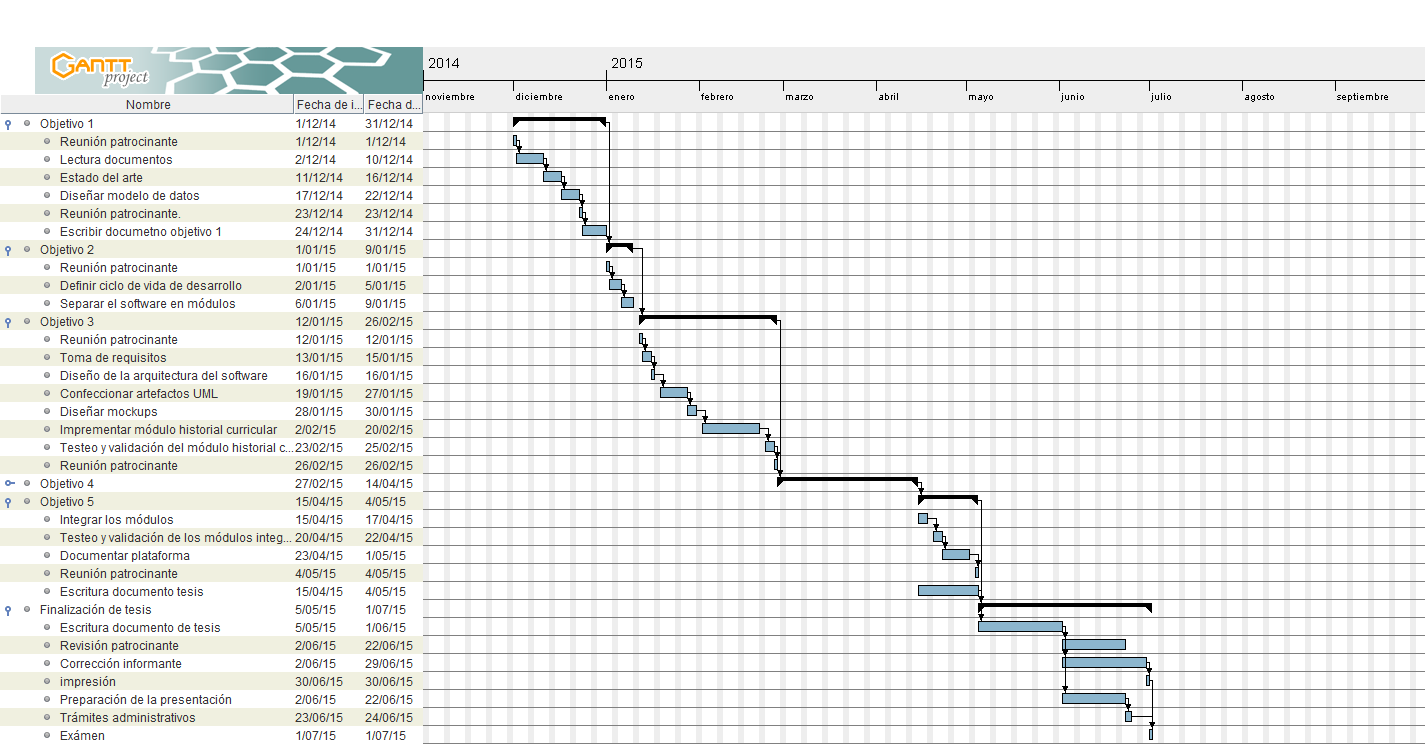
\includegraphics[width=1\textwidth]{images/Capitulo_3/carta_gantt.png}
		\caption[Carta Gantt que exhibe las etapas de desarrollo del sistema]{Carta Gantt que exhibe las etapas de desarrollo del sistema \footnote{}}
		\label{figura_cartaGantt}
	\end{figure}
	\footnotetext{Elaboración propia.}

	Durante el proceso de desarrollo del producto software es importante tener en cuenta lo siguiente:
	\begin{itemize}
		\item Es importante reunirse con el profesor patrocinante al comienzo, durante y al
		término de una iteración, para así aclarar y resolver requerimientos específicos del
		sistema que puedan surgir.
		\item El producto final se dará terminado cuando se hayan cumplido todos los requisitos
		del sistema.
	\end{itemize}

\subsection{Análisis}
	En esta sección se describen los requerimientos y casos de uso más representativos de cada módulo, los cuales fueron obtenidos y discutidos mediante  reuniones con el profesor patrocinador, con el objetivo de identificar los requisitos funcionales y no funcionales que deberían satisfacer el producto software final.
		
	\subsubsection{Requerimientos}
	A continuación se presenta una lista de los requisitos que se definieron para el producto software.

	\myparagraph{Requisitos funcionales}
	
	Los requisitos funcionales del sistema se presentan en la Tabla \ref{Tabla_requisitos_funcionales}.
	\\
	
	
	\begin{longtable}{l |p{11cm}}
	
		\caption{Requisitos funcionales}
		\label{Tabla_requisitos_funcionales}\\

		
		\hline
		\endfirsthead
		\multicolumn{2}{c}%
		{\tablename\ \thetable\ -- \textit{Continuación de la pagina anterior}} \\
		\hline
	
		\hline
		\endhead
		\hline \multicolumn{2}{r}{\textit{Continúa en la página siguiente}} \\
		\endfoot
		\hline
		\endlastfoot
		\rowcolor{LightBlue2} REQF-01 & Autentificación de usuario\\ \hline
		\textbf{Descripción} & El sistema debe ser capaz de diferenciar distintos tipos de usuarios, mediante el RUT, tipo de usuario y contraseña. Estos pueden ser de tres tipo: Administrador, Editor, y Subscriptor.\\ \hline \hline
		
		\rowcolor{LightBlue2} REQF-02 & Gestión de perfil\\ \hline
		\textbf{Descripción} & El sistema debe permitir que los usuarios puedan modificar su contraseña. Además  debe permitir que el Administrador pueda modificar los datos que el usuario ingresó al momento de registrarse.\\ \hline \hline
		
		\rowcolor{LightBlue2} REQF-03 & Desplegar historial curricular\\  \hline
		\textbf{Descripción} &El sistema debe permitir que  todos los usuarios  puedan ver el conjunto de hitos curriculares de una carrera en particular, mediante la facultad, la escuela y la carrera previamente ingresados por el usuario.\\  \hline \hline
		
		\rowcolor{LightBlue2} REQF-04 & Registro de usuarios\\ \hline
		\textbf{Descripción} & El sistema deberá permitir el registro de nuevos usuarios, los cuales deben ser creados por el Administrador. Los datos a solicitar son: RUT, nombre, apellido paterno, apellido materno, correo electrónico y rol. La contraseña será los 6 primeros dígitos del  RUT ingresado.\\ \hline
		
		\rowcolor{LightBlue2} REQF-05 & Gestión de documentos\\  \hline
		\textbf{Descripción} & El sistema debe permitir al Administrador y Editor crear nuevos registros curriculares, indicando el plan de estudio, la carrera y el tipo de hito: Modificación mayor, Modificación menor o Innovación Curricular, además  debe permitir subir uno o mas archivos en formato PDF por registros, los cuales el sistema los  tienen que clasificar en: Resolución, Comunicación Interna y Petición de requisitos.\\  \hline
		
		\rowcolor{LightBlue2} REQF-07 & Visor de PDF\\  \hline
		\textbf{Descripción} & El sistema debe permitir al usuario ver  cualquier documento que se encuentre almacenado en la base de datos.\\  \hline \hline
		
		
		\rowcolor{LightBlue2} REQF-08 & Notificaciones\\  \hline
		\textbf{Descripción} & El sistema desplegará distintos tipos de notificaciones al momento de realizar cualquier tipo de cambio (guardar, editar, eliminar). Los dos tipos de alertas que se consideraron en la plataforma web son : \textbf{Success} y \textbf{Error}. \\  \hline \hline
		
		\rowcolor{LightBlue2} REQF-09 & Almacenar bitácora de los usuarios\\  \hline
		\textbf{Descripción} & El sistema internamente debe almacenar todas las notificaciones de los eventos ocurridos en la plataforma a fin de tener un registro de  todas  las actividades  que realizan los usuarios en la plataforma. Un registro de la bitácora debe tener necesariamente esta compuesto por: Código de la alerta, mensaje de la alerta, fecha y el RUT de usuario quien ejecutó dicha alerta.\\  \hline
		
		\rowcolor{LightBlue2} REQF-10 & Visualización de bitácora\\  \hline
		\textbf{Descripción} & El sistema debe permitir al administrador visualizar todos los eventos ocurridos en el sistama.\\ 
	
	\end{longtable}

	\myparagraph{Requisitos no funcionales}
	Los requisitos no funcionales se presentan en la Tabla \ref{Tabla_requisitos_no_funcionales}.
	\\

	\begin{longtable}{l |p{11cm}}
		
		\caption{Requisitos no funcionales}
		\label{Tabla_requisitos_no_funcionales}\\
		
		
		\hline
		\endfirsthead
		\multicolumn{2}{c}%
		{\tablename\ \thetable\ -- \textit{Continuación de la pagina anterior}} \\
		\hline
		
		\hline
		\endhead
		\hline \multicolumn{2}{r}{\textit{Continúa en la página siguiente}} \\
		\endfoot
		\hline
		\endlastfoot
	
			\rowcolor{LightBlue2} REQNF-01 & Ambiente Web\\ \hline
			\textbf{Descripción} & El sistema debe visualizarse y funcionar correctamente en cualquier navegador, especialmente en Internet Explorer, Mozilla y Google Chrome.\\ \hline \hline
			
			\rowcolor{LightBlue2} REQNF-02 & Escalabilidad\\ \hline
			\textbf{Descripción} & El sistema debe estar en capacidad de permitir en el futuro el desarrollo de nuevas funcionalidades, modificar o eliminar funcionalidades.\\  \hline
			
			\rowcolor{LightBlue2} REQNF-03 & Facilidad de uso\\ \hline
			\textbf{Descripción} & La interfaz del sistema debe ser amigable con el usuario, Mensajes de errores y éxito.\\ \hline
			
	
			
			\rowcolor{LightBlue2} REQNF-04 & Facilidad de pruebas\\ \hline
			\textbf{Descripción} & El sistema debe contar con facilidad para la identificación de la localización de los errores durante la etapa de prueba.\\ \hline \hline
			
			\rowcolor{LightBlue2} REQNF-05 & Validación\\ \hline
			\textbf{Descripción} & El sistema tiene que poseer una interfaz en la cual se validen los campos obligatorios y  manejo de datos que se ingresan.\\ 
	\end{longtable}

	\subsubsection{Modelo conceptual}
	Para facilitar la compresión de la problemática que se desea solucionar mediante el producto software, en la Figura \ref{Figura_Modelo_conceptual}  se presenta un modelo conceptual, que muestra el dominio dentro del cual se encuentra inmerso el proyecto.
	\\
		\begin{figure}[H]
			\centering
			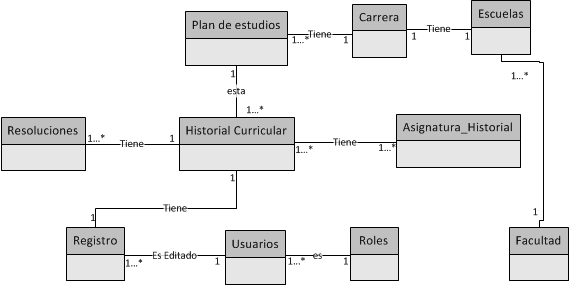
\includegraphics[width=1\textwidth]{images/Capitulo_3/Modelo_Conceptual.png}
			\caption[Modelo conceptual del proyecto]{Modelo conceptual del proyecto \footnote{}}
			\label{Figura_Modelo_conceptual}
		\end{figure}
		\footnotetext{Elaboración propia.}
	\subsubsection{Casos de uso}
	En las Figuras \ref{caso_uso_Administrador}, \ref{caso_uso_Editor}, \ref{caso_uso_Suscriptor} se presentan los diferentes casos de uso para los actores
	involucrados en el sistema.
	
	
	\begin{figure}[H]
		\centering
		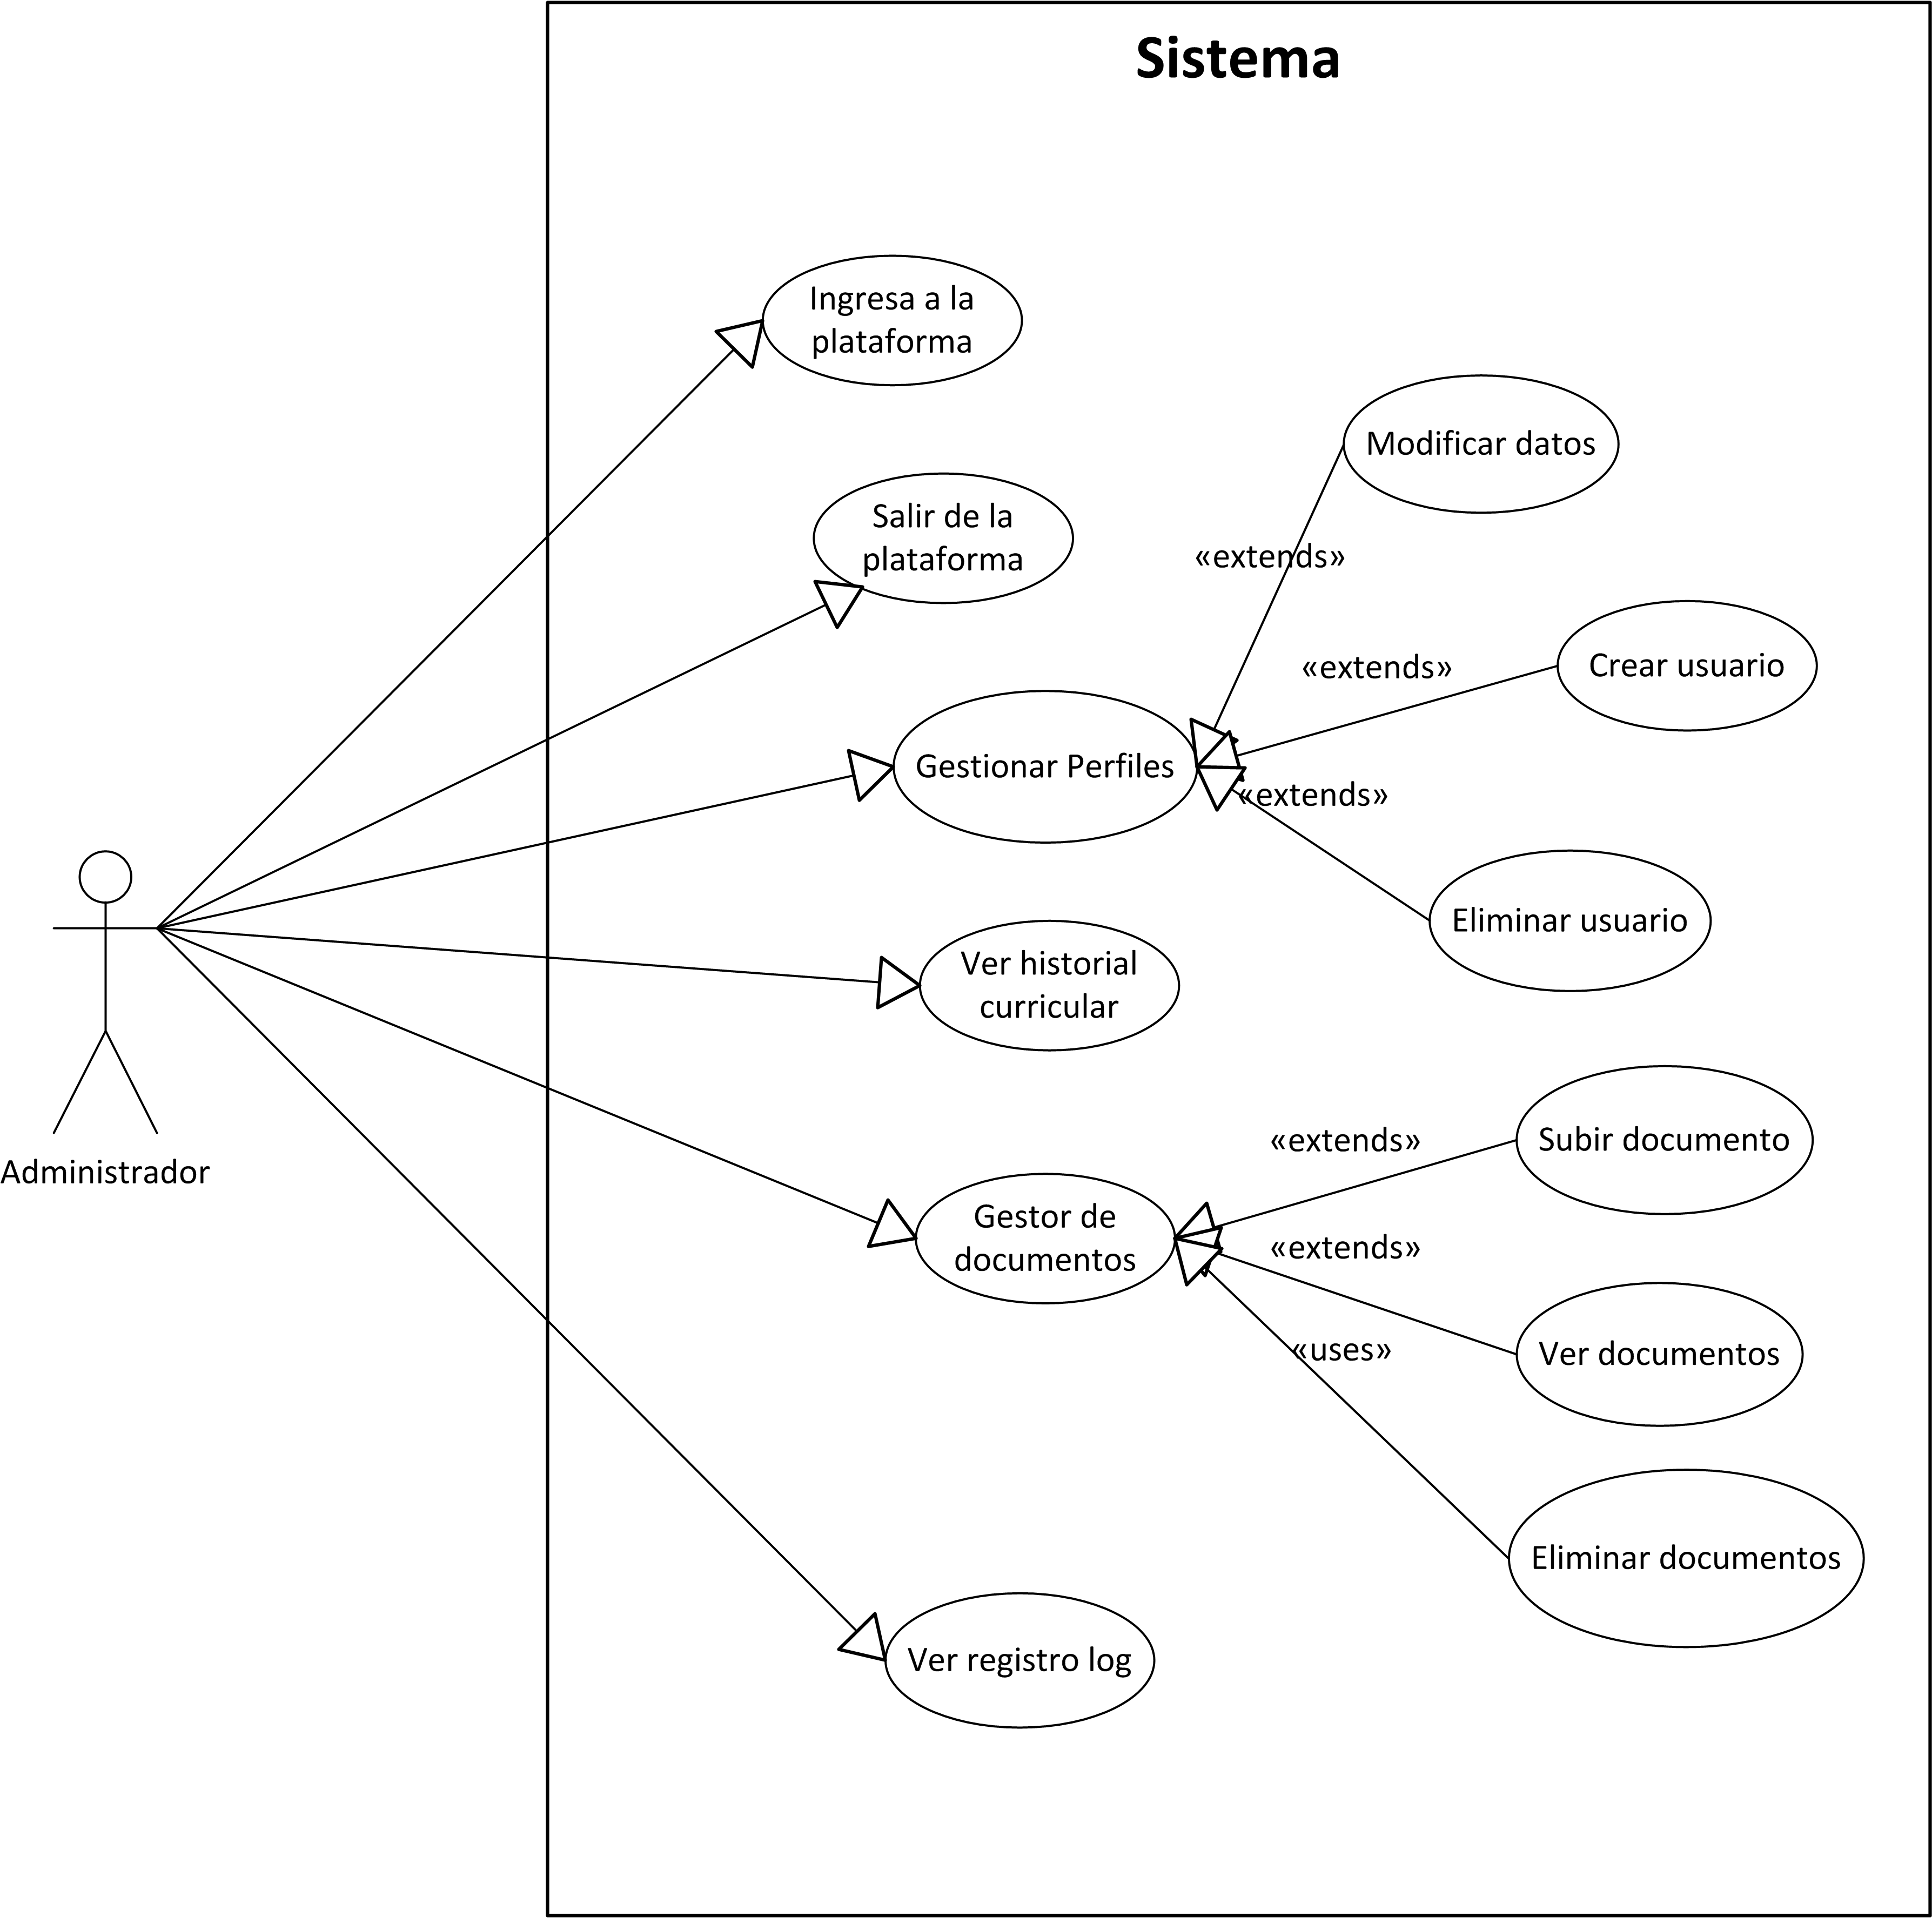
\includegraphics[width=1\textwidth]{images/Capitulo_3/caso_uso_Administrador.png}
		\caption[Diagrama de caso de uso para el Administrador]{Diagrama de caso de uso para el Administrador \footnote{}}
		\label{caso_uso_Administrador}
	\end{figure}
	\footnotetext{Elaboración propia.}
	
	\begin{figure}[H]
		\centering
		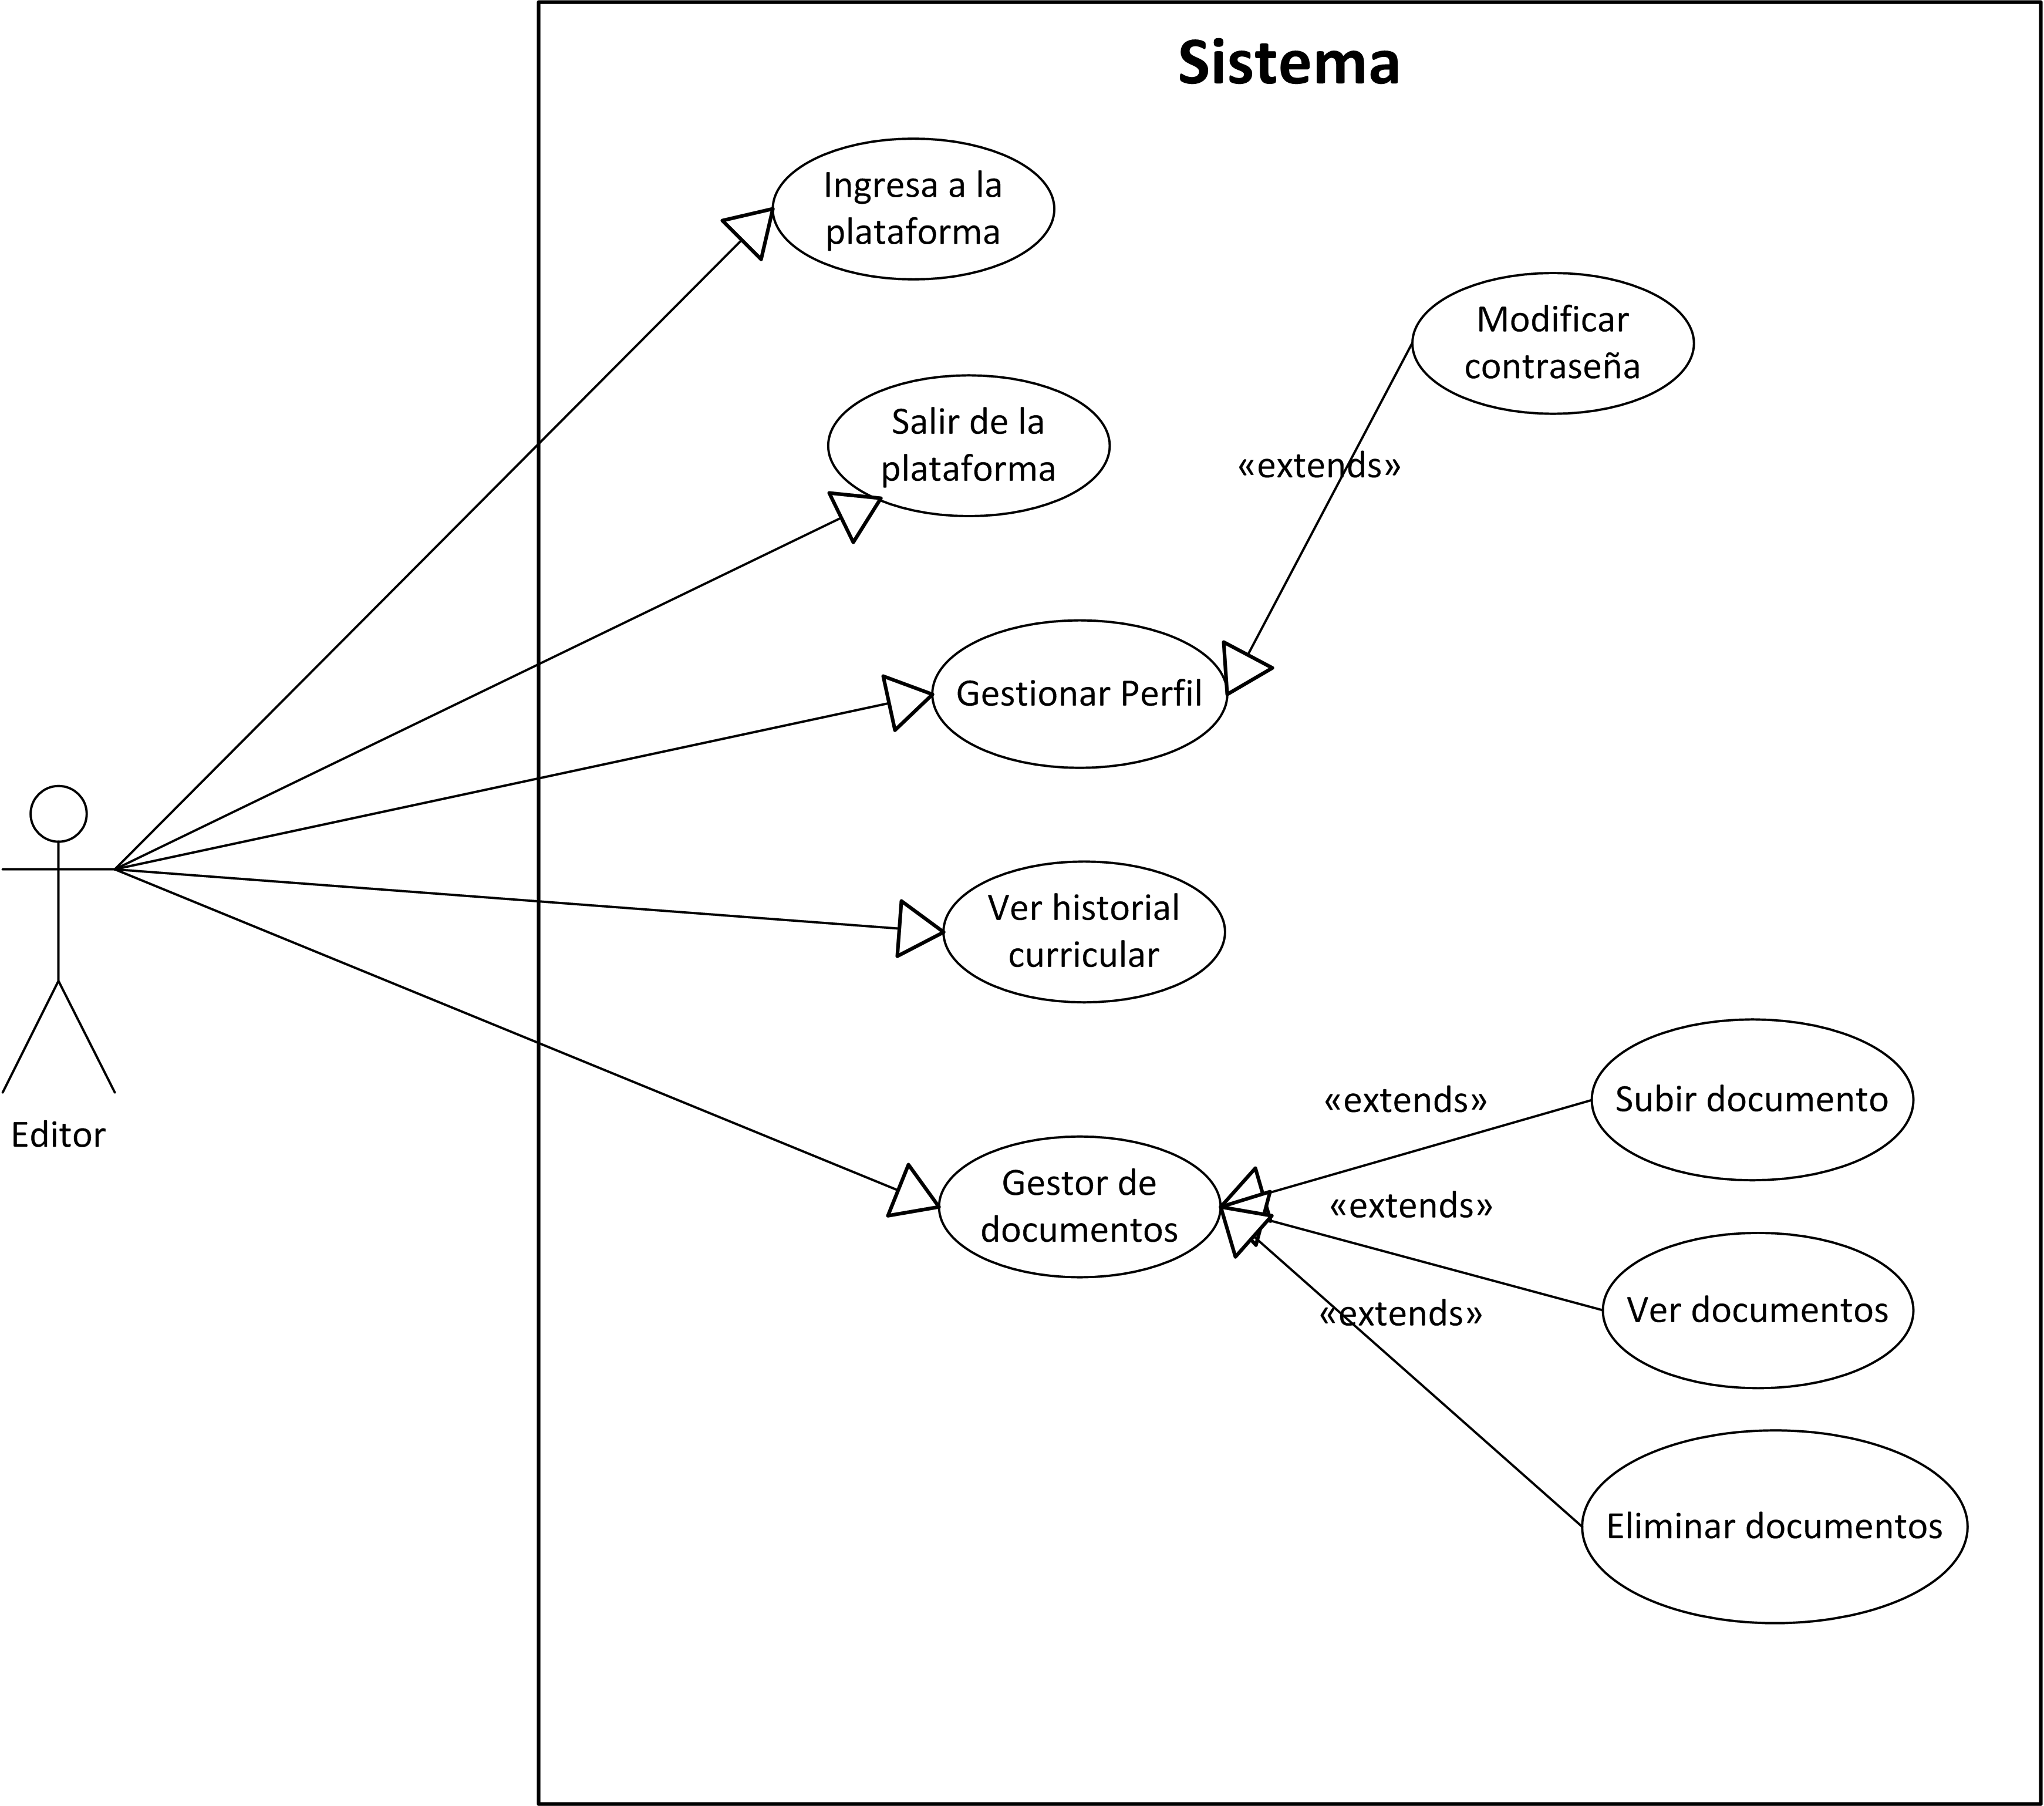
\includegraphics[width=1\textwidth]{images/Capitulo_3/caso_uso_Editor.png}
		\caption[Diagrama de caso de uso para el Editor]{Diagrama de caso de uso para el Editor \footnote{}}
		\label{caso_uso_Editor}
	\end{figure}
	\footnotetext{Elaboración propia.}
	
	\begin{figure}[H]
		\centering
		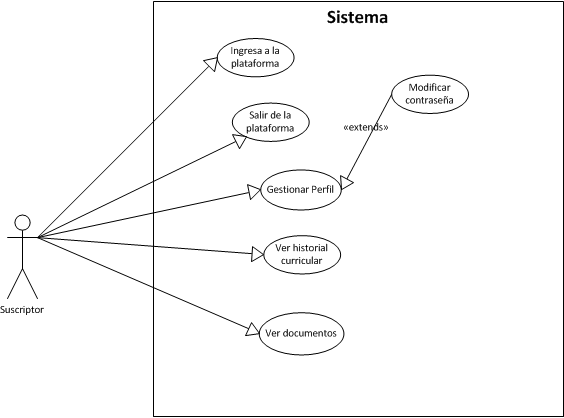
\includegraphics[width=1\textwidth]{images/Capitulo_3/caso_uso_Suscriptor.png}
		\caption[Diagrama de caso de uso para el Suscriptor]{Diagrama de caso de uso para el Suscriptor \footnote{}}
		\label{caso_uso_Suscriptor}
	\end{figure}
	\footnotetext{Elaboración propia.}
	
	\myparagraph{Descripción de los actores del sistema} \label{usuarios_Sistema}
	
	
	\textbf{Suscriptor:} corresponde al grupo de individuos que pueden revisar los datos en la plataforma, es decir, pueden ver el historial curricular de una carrera y ver todas las resoluciones. sin embargo no posee ningún permiso de edición o creación.
	\\
	
	\textbf{Editor:} Este grupo de individuos posee todos los permisos necesarios para poder realizar todas las operaciones básicas (crear, leer,editar y borrar) sobre los registros curriculares y/o los documentos que están en el sistema.
	\\
	
	\textbf{Administrador:} Corresponde al individuo o grupo de individuos que tiene todas las
	funciones de un creador de registros curriculares, pero que además es el encargado de administrar la
	totalidad de usuarios de la plataforma, lo cual incluye el registro, edición y eliminación
	de usuarios.
	
	
	
\subsection{Diseño e implementación}

	En esta sección se describe el diseño y la implementación para los módulos: \textit{Historial curricular} y \textit{Gestor de documentos} de la plataforma. En un principio se muestran algunos artefactos generales correspondientes al diagrama de componentes y al modelo de datos. Posteriormente para cada módulo se presentaran los casos de uso, además del diagrama de secuencia correspondiente, y un diagrama de pantallas para ver la interacción del caso de uso con el resto del sistema.


	\subsubsection{Diagramas de componentes}
	\subsubsection{Modelo de datos}
	
	El contexto en el que se desenvuelve el software contempla 14 entidades, de las cuales 8 de ellas se exportaron desde la base de datos de la Universidad para poder trabajar en un ambiente de desarrollo, estas entidades son: Facultad, Escuelas, Carreras, PlanEstudio, PlanAsignatura, Plan\_asig\_requisito,institutos y asignaturas.
	\\
	
	Las entidades restantes fueron creadas con el fin de satisfacer las necesidades de la problemática en la cual se encuentra inmerso en proyecto. El modelo de datos completo se puede ver en la Figura \ref{Modelo_E_R}.
	\\
	
	\begin{figure}[H]
		\centering
		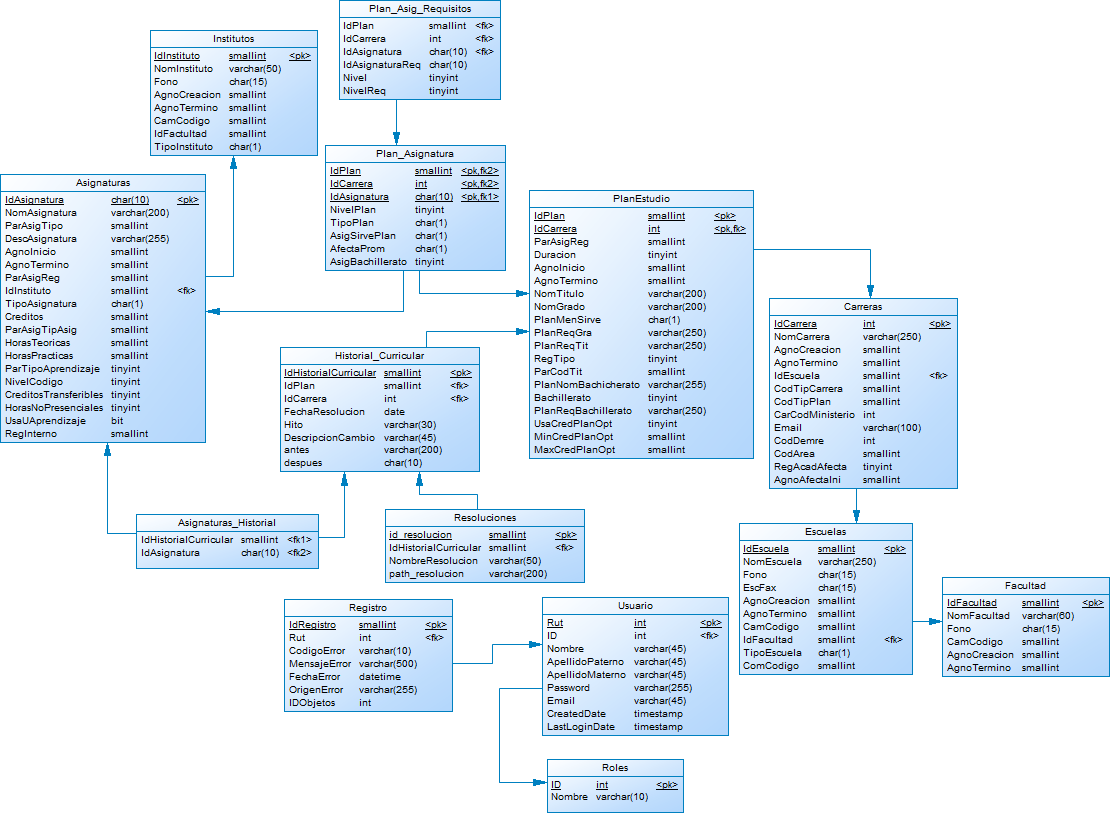
\includegraphics[width=1\textwidth]{images/Capitulo_3/Modelo_E_R.png}
		\caption[Modelo de datos Entidad-Relación]{Modelo de datos Entidad-Relación \footnote{}}
		\label{Modelo_E_R}
	\end{figure}
	\footnotetext{Elaboración propia.}
	\subsubsection{Módulo historial curricular}
	
	El módulo historial curricular esta diseñado para que todos los usuarios definidos en la Sección \ref{usuarios_Sistema} tengan acceso a él, a causa de que su principal objetivo es ver la trazabilidad de una carrera en particular.
	\myparagraph{Diseño}
	A continuación se describe el diseño del caso de uso más significativo para el módulo  historial curricular de la plataforma, que corresponde a la visualización de la trazabilidad de los planes de estudio de las carreras . Se presentará en detalle la composición de este caso de uso y su participación en el sistema.
		
	\mysubparagraph{ Caso de uso real más significativo} 
	
	El caso de uso “Ver historial curricular” ocurre cuando un usuario  desea  ver los cambios que curriculares que se le han aplicado a una carrera en particular. El caso de uso real “Ver historial curricular” se presenta en la Tabla \ref{Tabla_Caso_Uso_ver_historial}.
	
	
		\begin{longtable}{l| p{11cm}}
			
			\caption{Caso de uso Ver historial curricular}
			\label{Tabla_Caso_Uso_ver_historial}\\
			
			
			\hline
			\endfirsthead
			\multicolumn{2}{c}%
			{\tablename\ \thetable\ -- \textit{Continuación de la pagina anterior}} \\
			\hline
			
			\hline
			\endhead
			\hline \multicolumn{2}{r}{\textit{Continúa en la página siguiente}} \\
			\endfoot
			\hline
			\endlastfoot
			\rowcolor{LightBlue2}  \multicolumn{2}{c}{Caso de Uso Ver Historial Curricular} \\ 
			
			
			\textbf{Actores} & Administrador, Editor, Suscriptor.\\ \hline
			
			\textbf{Propósito} & Visualizar los cambios curriculares que se han realizado en una determinada carrera.\\ \hline
			
			\textbf{tipo} & Primario y esencial\\ \hline
			
			\multicolumn{2}{l}{\textbf{Resumen:}sfgsdfg} \\  \hline
			 
			\rowcolor{LightBlue2}  \multicolumn{2}{c}{Interfaz: Formulario Ver Historial Curricular} \\  \hline \hline
			
			\multicolumn{2}{c}{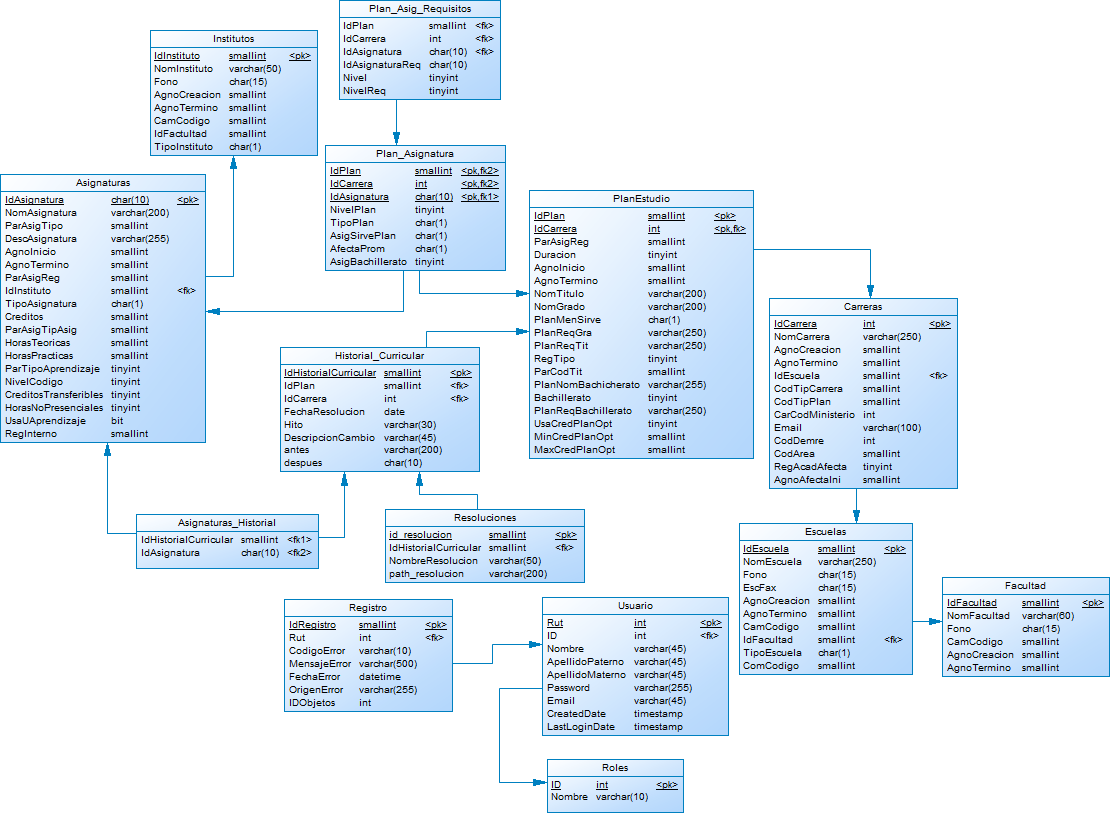
\includegraphics[width=1\textwidth]{images/Capitulo_3/Modelo_E_R.png}} \\ 
		
		\end{longtable}
	\subsubsection{Metodología}
	
\subsection{Validación del software}

